\documentclass[10pt]{beamer}
\usepackage[utf8]{inputenc}
\usepackage{graphicx}
\usepackage{amssymb}
\usepackage{amsmath}
\usepackage[backend=bibtex,style=ieee,bibencoding=ascii,sorting=none]{biblatex}
\addbibresource{refs}
\usetheme{Madrid}
\usecolortheme{default}


\title{Hopfield Networks }
\author[STAT 9100]{Carlos Martinez-Villar}
\date{May 5, 2022}

\begin{document}

\begin{frame}
	\titlepage
\end{frame}

%%%%%%%%%%%%%%%%%%%%%%%%%%%%%%%%%%%%%%%%%%%%%%%%%%%%%%%%%%%%%
% MODEL
%%%%%%%%%%%%%%%%%%%%%%%%%%%%%%%%%%%%%%%%%%%%%%%%%%%%%%%%%%%%%
%\begin{frame}{Model}
%	
%\end{frame}

\begin{frame}{Model --Why?, Neurophysiology, etc.}
	\begin{itemize}
		\item Often referred to as "content-addressable memory" or (more recently) "dense associative memory" system. 
		\item Similarities to Ising's model: overall state of the model is defined by individual states pointing in some direction (-1 or 1), and each individual state depends on its neighbors -- explicit in the original paper
		\item Proposed by Hopfield in 1982 with  "Neural networks and physical systems with emergent collective computational abilities" \cite{hopfield1982neural}. Hopfield (1984) \cite{hopfield1984neurons} considered the continuous case 
		\item Hebbian Learning:  $w_{ij} =  V^s_i V^s_j$
			\begin{itemize}
				\item "Neurons that fire together wire together" - attributed to Hebb \cite{hebb2005organization}
				\item A neurophysiological intuition is exploited so \emph{association} between neurons that can be used to determine connections among them
			\end{itemize}		
	\end{itemize}
\end{frame}

\begin{frame}{Model}	
	\centering
	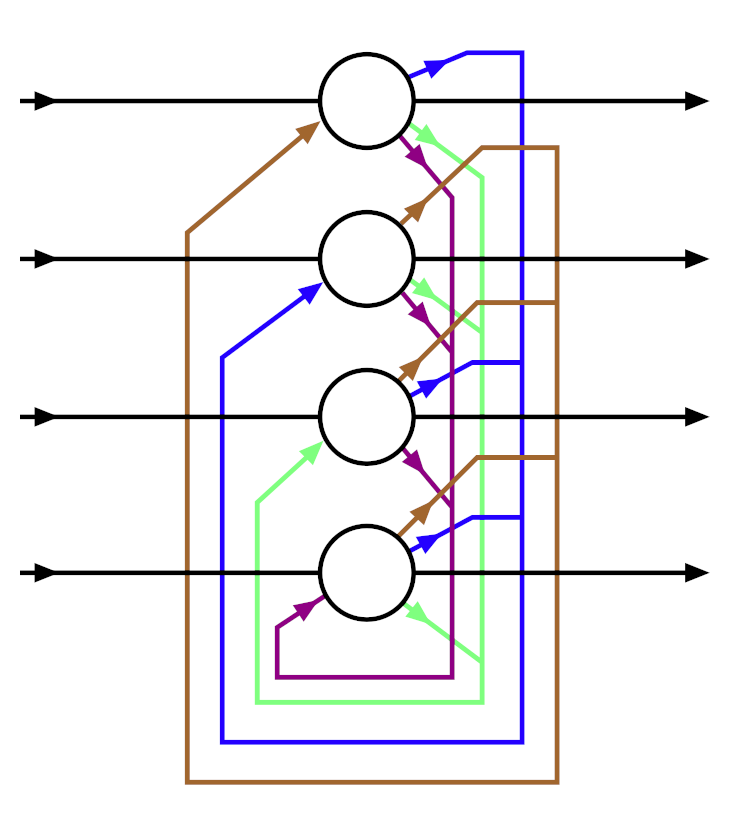
\includegraphics[width=0.8\textheight]{"../img/hopfieldnet.png"}
\end{frame}

\begin{frame}{Model -- Creating memories}	

	At a given state $s$ the weights of the network are 
	\begin{equation}
		w_{ij} = V^s_i V^s_j
	\end{equation}
	We can "learn" a set of target network states (memories) $ V^{(1)}, ..., V^{(M)}$ by setting weights of the network as the average over these memories:
	
		
	%equation for W
	\begin{equation}
		w_{ij} = \frac{1}{M} \sum^{M}_{1} V_i V_j
	\end{equation}

	with $w_{ii} = 0$. Or alternatively,
	\begin{equation}
	W = VV^T - I
	\end{equation}


%	\begin{itemize}
%		\item In the discrete case, memories can be stored as a binary vector in $\left{-1,1\right}$
%		\item Each element $v_i$ in this vector represents the state of a node/neuron $i$ in the network
%	\end{itemize}
%			
\end{frame}

\begin{frame}{Model -- Retrieving memories}

 	Each node is updated as 
    \begin{equation}
    V_i = 
    \left\{
        \begin{array}{lr}
           \ \   1 & \text{if } \sum^{}_{j} w_{ij} V_i > 0\\
            -1 & \text{otherwise} 
        \end{array}
    \right\} 
    \end{equation}

	Energy of the system (entropy?):
    	\begin{equation}
        		E = -\sum^{}_{i}s_i b_i - \sum^{}_{i \neq j}s_i s_j w_{ij}
    	\end{equation}
	
	Marginal changes for each node:	
    	\begin{equation}
 	       \Delta E_i = b_i + \sum s_j w_{ij}
     	\end{equation}
	

	
	\begin{itemize}
	\item Memories considered minima in the energy space of the network
	\item Ideally, since the system will consistently move towards a lower energy state, it should eventually retrieve a memory
	\end{itemize}
\end{frame}

\begin{frame}
	Hopfield (1984):\\
	\centering
	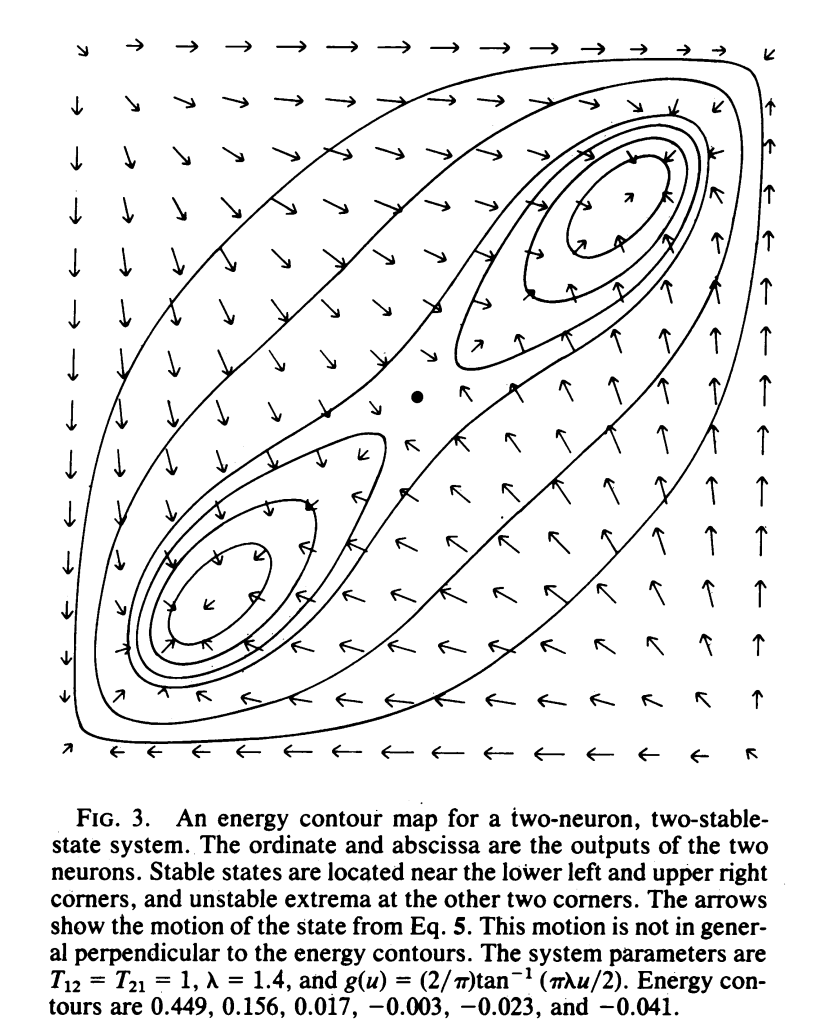
\includegraphics[width=0.5\textwidth]{"../img/hopfield_phase_space.png"}
\end{frame}


%%%%%%%%%%%%%%%%%%%%%%%%%%%%%%%%%%%%%%%%%%%%%%%%%%%%%%%%%%%%%
% VECTORS
%%%%%%%%%%%%%%%%%%%%%%%%%%%%%%%%%%%%%%%%%%%%%%%%%%%%%%%%%%%%%
\begin{frame}{Experiments (so far...) -- Hamming Distance}
	Hamming distance:
	\begin{equation}
		\sum^{N}_{i=1} I(x_i  \neq y_i)
	\end{equation}
	\begin{itemize}
		\item Distance between network  state and an original memory.
		\item Distance between perturbed memories/states and original memories
		\item i.e.: Any two binary states
	\end{itemize}
\end{frame}

\begin{frame}{Experiments (so far...) -- Simple state vectors}	
	\centering
	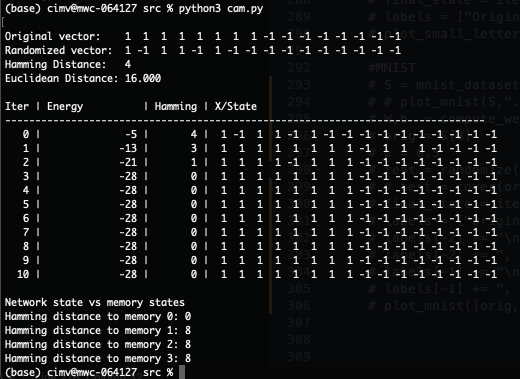
\includegraphics[width=0.8\textwidth]{"../img/log_vector_good.png"}	
\end{frame}

\begin{frame}{Experiments (so far...) -- Simple state vectors}	
	\centering
	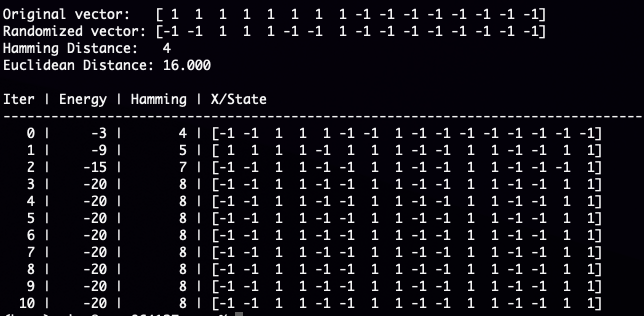
\includegraphics[width=0.8\textwidth]{"../img/log_vector_spurious.png"}
\end{frame}




%%%%%%%%%%%%%%%%%%%%%%%%%%%%%%%%%%%%%%%%%%%%%%%%%%%%%%%%%%%%%
% LETTERS 
%%%%%%%%%%%%%%%%%%%%%%%%%%%%%%%%%%%%%%%%%%%%%%%%%%%%%%%%%%%%%
\section{Experiments and Code}

\begin{frame}{Experiments (so far...)}	
	\centering
	
\includegraphics[width=0.8\textwidth]{"../img/small_letters.png"}
\end{frame}

\begin{frame}{Experiments (so far...)}	
	\centering
%	
\includegraphics[width=0.8\textwidth]{"../img/small_letters.png"}
	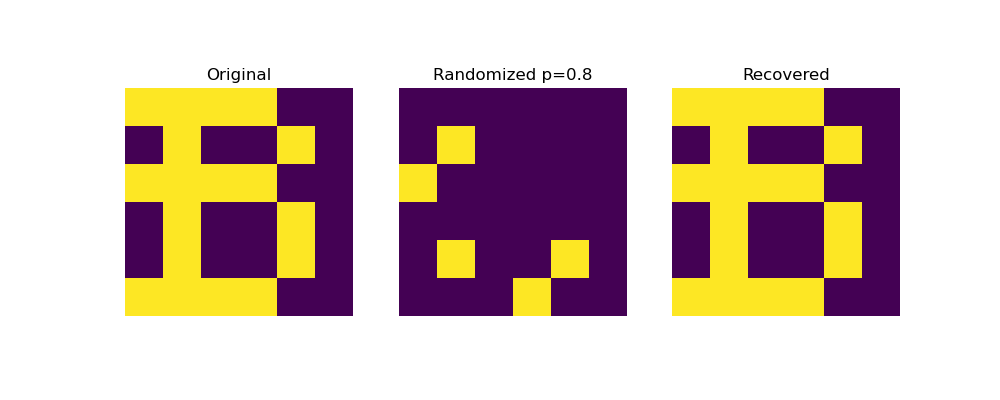
\includegraphics[width=0.8\textwidth]{"../img/letters_result_B.png"}	
	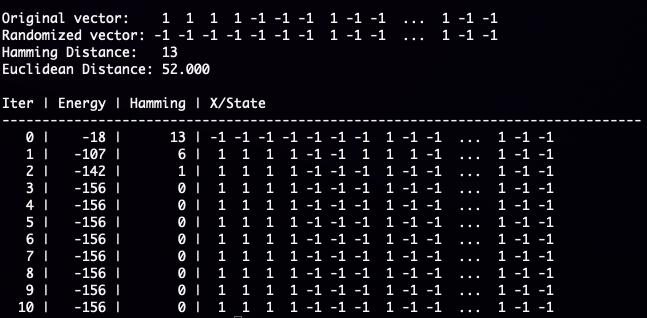
\includegraphics[width=0.5\textwidth]{"../img/log_letter_B.png"}

\end{frame}

\begin{frame}{Experiments (so far...)}	
	\centering
	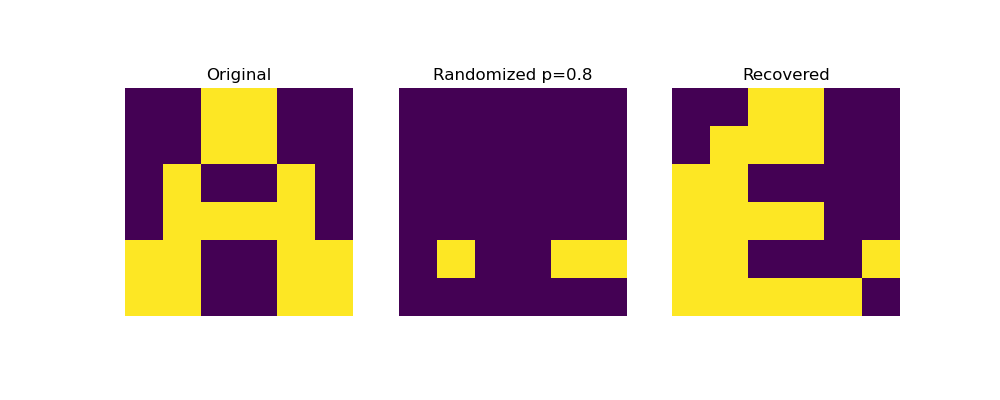
\includegraphics[width=0.8\textwidth]{"../img/letters_result_A.png"}
	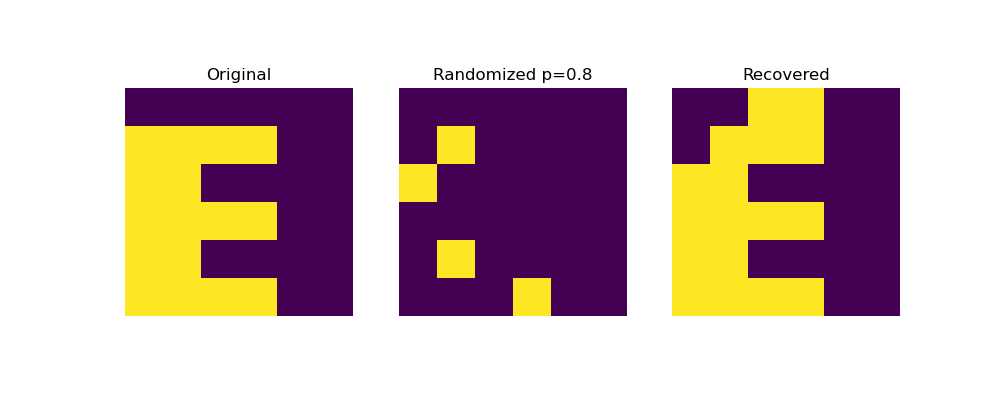
\includegraphics[width=0.8\textwidth]{"../img/letters_result_E.png"}	
\end{frame}

%%%%%%%%%%%%%%%%%%%%%%%%%%%%%%%%%%%%%%%%%%%%%%%%%%%%%%%%%%%%%
%DIGITS MNIST
%%%%%%%%%%%%%%%%%%%%%%%%%%%%%%%%%%%%%%%%%%%%%%%%%%%%%%%%%%%%%
\begin{frame}{Experiments (so far... ) -- MNIST}	
	\centering
	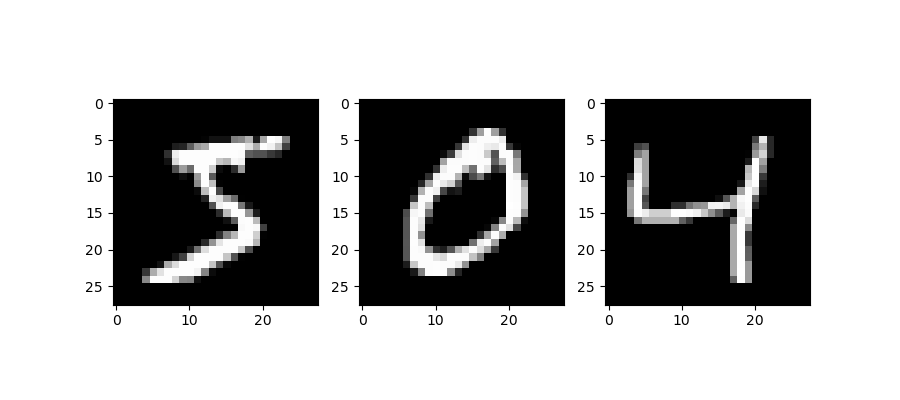
\includegraphics[width=0.75\textwidth]{"../img/digits.png"}\\
	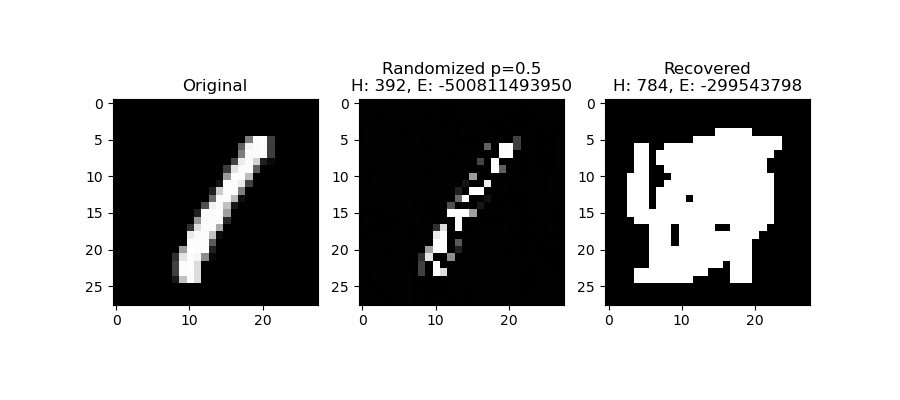
\includegraphics[width=0.75\textwidth]{"../img/digits_result_grayscale.png"}	
\end{frame}

\begin{frame}{Experiments (so far...) -- MNIST}	
	\centering
	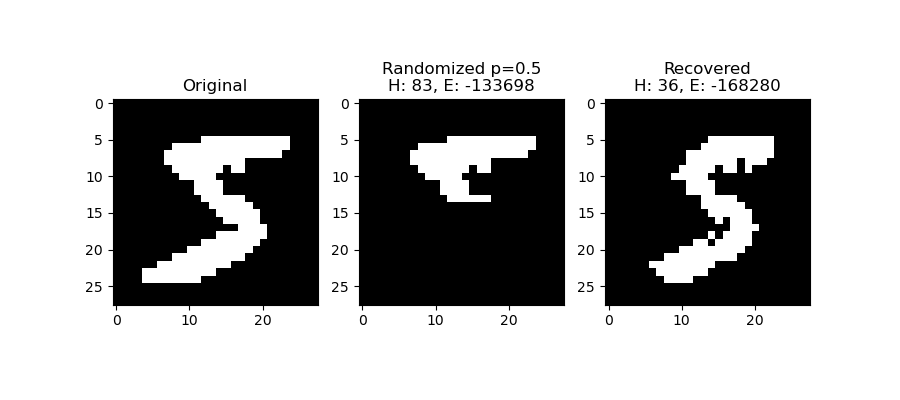
\includegraphics[width=0.75\textwidth]{"../img/digits_result_good_covered.png"}\\
	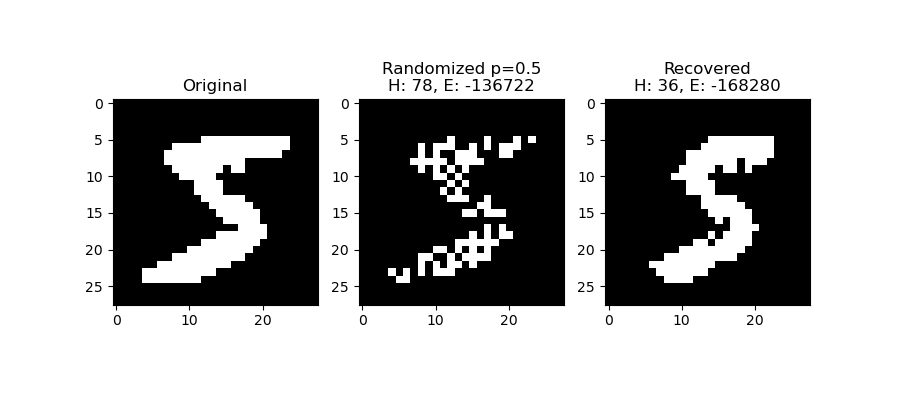
\includegraphics[width=0.75\textwidth]{"../img/digits_result_good_random.png"}
\end{frame}

\begin{frame}{Experiments (so far...) -- MNIST}	
	\centering
	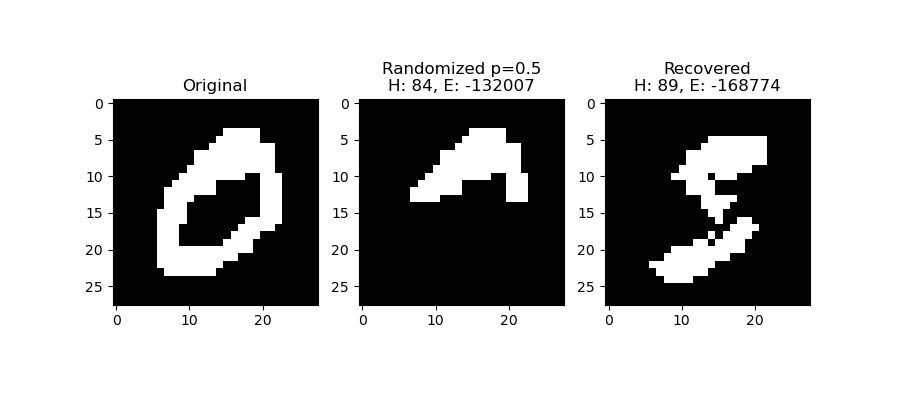
\includegraphics[width=0.75\textwidth]{"../img/digits_result_bad_covered.png"}\\
	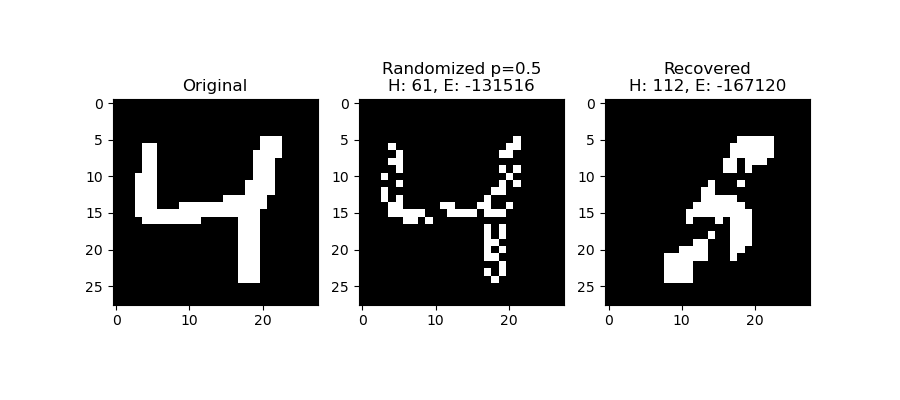
\includegraphics[width=0.75\textwidth]{"../img/digits_result_bad_random.png"}
\end{frame}


\begin{frame}{Next Steps}
	\begin{itemize}
		\item Simplest forms of Hopfield Networks are too prone to local minima or spurious states
		\item Good approximation for optimization problems that use other graphical models \cite{mackay2003information}.
		\item Two (maybe three) routes:
			\begin{itemize}
				\item Discrete "Modern Hopfield Networks": far greater capacity, more general (in their mathematical expression) \cite{krotov2016dense}
				\item Application of Ising models to a particular dataset later to be tested against Hopfield Net.
				\item Stochastic activation function on traditional Hopfield
				\item Last two options will likely emphasize the model as a tool for inference and/or comparison with models studied in class
			\end{itemize}
	\end{itemize}
\end{frame}

\begin{frame}{References}
	\printbibliography
\end{frame}

\end{document}